\chapter{2D Segmentation}

In this chapter, we establish the task of 2D Segmentation of EM images, attempt to train models that perform well on this task, and evaluate our results. The purpose of these experiments is not so much to achieve state-of-the-art performance on the task, but to examine the effect that increasing training data quality and reducing variance in predictions has on model performance.

\section{Task Definition}

2D Segmentation involves taking a single 2D slice of EM tissue and segmenting it into its constituent cells. Compared to 3D segmentation, this is a simple task, but will still allow us to show the properties of different models on EM data. To achieve segmentation, we will train models that predict boundaries of cells, and then use a Watershed algorithm to segment based on those boundary predictions.

The problem statement for 2D Boundary detection is such: given a 2-dimensional single-channel (i.e. greyscale) image of neural tissue taken with an electron microscope, produce an image that labels the boundaries of all the distinct cells in the image. An example of this boundary-detection task can be found in Figure \ref{fig:isbi_example}. This task is made somewhat more difficult by the existence of organelles with well-defined borders, as well as blood vessels and structured interstitial tissue.

\begin{figure}
    \centering
	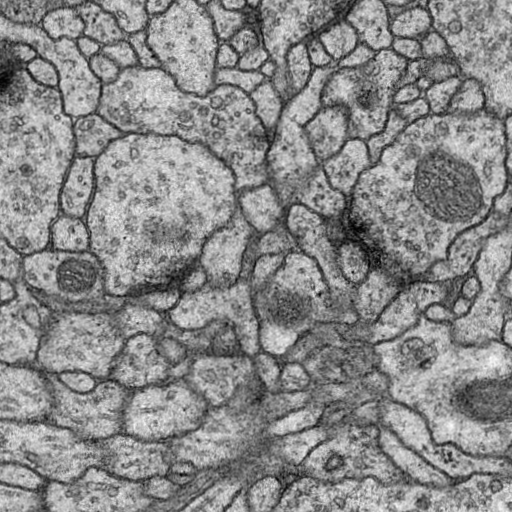
\includegraphics[width=0.33\textwidth]{img/isbi_raw_example}
	\hspace{1cm}
	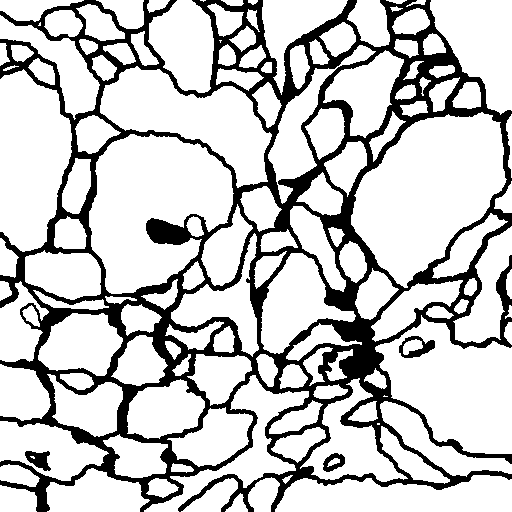
\includegraphics[width=0.33\textwidth]{img/isbi_label_example}
    \caption[An example of 2D boundary detection]{An example of 2D boundary detection. Left: the original image taken with an electron microscope. This particular example is neuron tissue taken from \textit{Droposphila melanogaster} in a dataset created for the ISBI 2012 EM segmentation challenge \cite{Arganda-Carreras2015}. The resolution of each pixel is 4nm x 4nm. Right: The ground truth boundaries corresponding to cell membranes in the input image, as labeled by human experts. The labels are binary values, although the actual border deliniation is somewhat arbitrary due to the fact that real applications of boundary detection are invariant to small differences in boundary shapes.}
    \label{fig:isbi_example}
\end{figure}

\section{Evaluation Metrics}

The two main evaluation metrics we will use for this task are Rand Error and Pixel Error. Formal definitions of both of these error metrics can be found in Appendix A. 

\begin{itemize}
\item \textbf{Rand Error}: We will use the Rand Error to determine whether or not the segmentation process correctly labels different cells as different objects. We will also look at the Rand Split Error and the Rand Merge Error, to see where the models inaccurately split and merge different regions.
\item \textbf{Pixel Error}: We will use the Pixel Error to gauge the efficacy of our models at predicting the intermediate boundary stage.
\end{itemize}

\section{Models}

We define two models - both closely resembling models from the literature -  with which we will run experiments:

\begin{itemize}
\item \textbf{N4}
\item \textbf{VD2D}
\end{itemize}

\section{Dataset}

\TODO{Talk about splits}

One prominent competition that evaluates performance on this sort of task is the International Symposium on Biomedical Imaging (ISBI) EM Segmentation Challenge, which has had active submission since 2012. The ISBI Challenge organizers provides a training set of EM images, along with a set of binary boundary maps. The challenge website describes the training data as \quotes{a set of 30 sections from a serial section Transmission Electron Microscopy (ssTEM) data set of the Drosophila first instar larva ventral nerve cord (VNC). The microcube measures 2 x 2 x 1.5 microns approx., with a resolution of 4x4x50 nm/pixel}\cite{Arganda-Carreras2015}. This resolution description implies that each pixel represents a 4x4nm patch on the surface of a slice, with each slice being 50nm thick. We build prediction systems using several different architectures, regularization methods, and data transformation techniques. We make several submissions to the leaderboard, ultimately scoring quite competitively.

\section{Training}

\section{Results}

\begin{table}
\centering
	\begin{tabular}{lllll}
\toprule
{} & Pixel Error & Rand - Full & Rand - Merge & Rand - Split \\
\midrule
N4 w/o aug   &    0.112204 &     0.65693 &     0.506545 &     0.934315 \\
N4           &   0.0827646 &    0.950296 &     0.933164 &     0.968069 \\
VD2D w/o aug &   0.0998995 &     0.80245 &     0.725266 &     0.898018 \\
VD2D         &   0.0842352 &    0.954286 &     0.976404 &     0.933148 \\
VD2D (x5)    &    0.083214 &    0.975745 &     0.985624 &     0.968843 \\
\bottomrule
\end{tabular}

	\caption[Results of 2D Segmentation]{The results of various architectures on the 2D Segmentation task. Notice that using data augmentation drastically improves the performance of the nets. Additionally, ensembling multiple instances of the best architecture produces the best Rand Score.}
	\label{tab:2d_results}
\end{table}

\begin{figure}
\centering
\textbf{Rand Index}
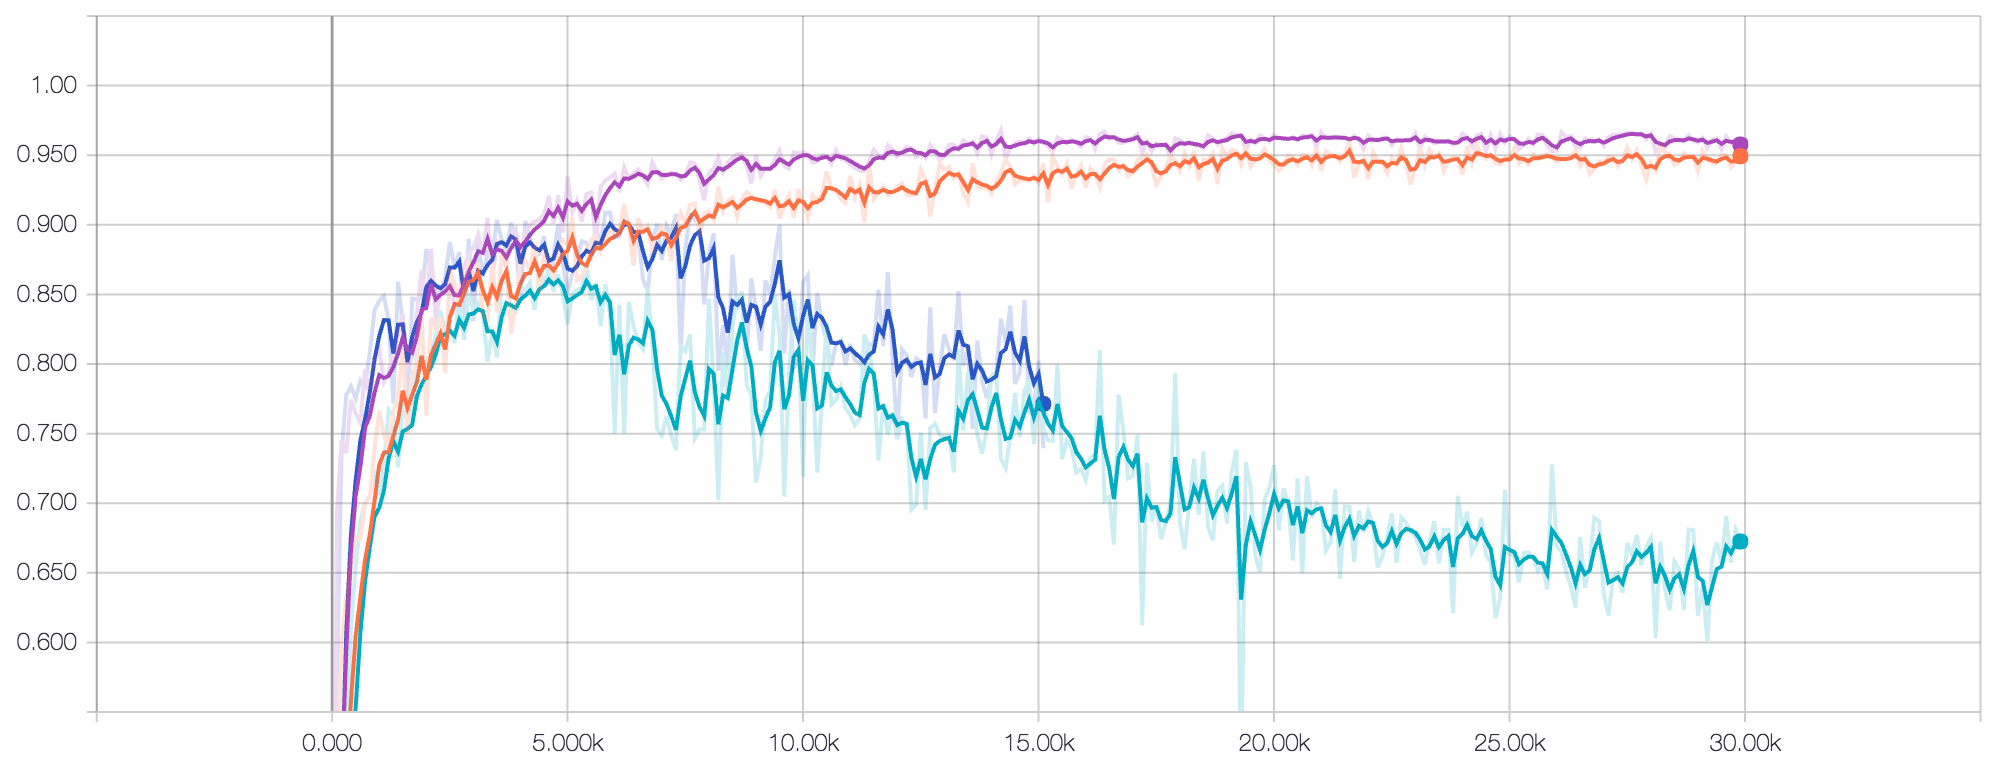
\includegraphics[width=\textwidth]{img/2d_rand.png} \\
\textbf{Pixel Error}
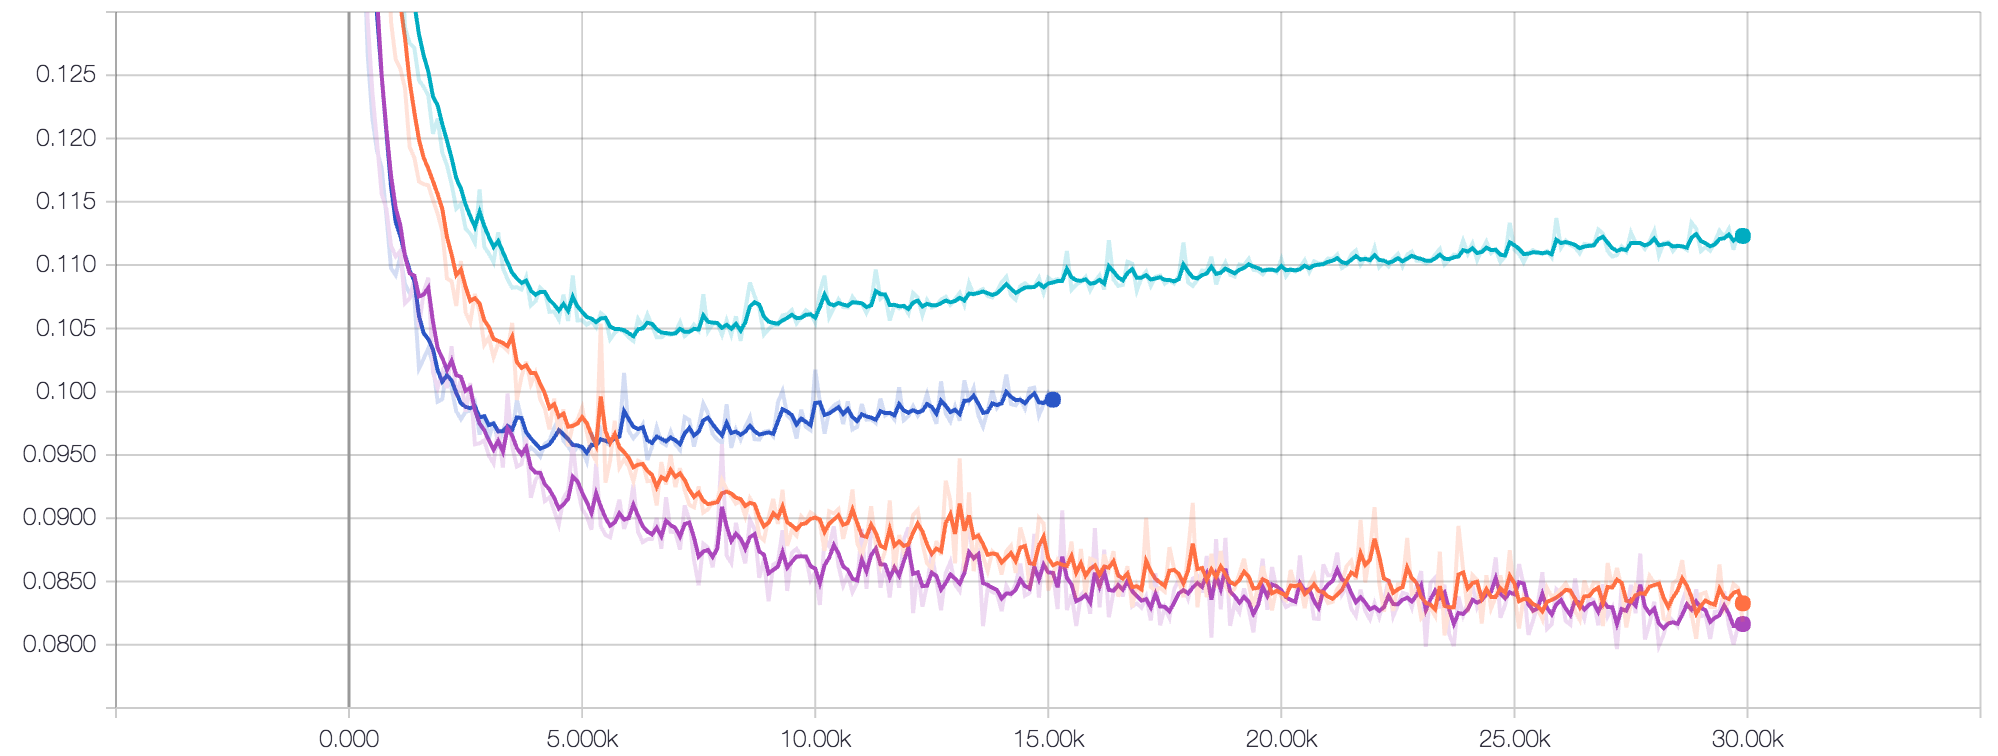
\includegraphics[width=\textwidth]{img/2d_pixel.png}
\label{fig:training_curves}
\caption[Training curves for 2D segmentation]{Training curves, smoothed, for 2D segmentation. Top: The full Rand scores on the validation set (from top: VD2D, N4, VD2D w/o augmentation, N4 w/o augmentation). Bottom: The pixel error on the validation set (from top: N4 w/o augmentation, VD2D w/o augmentation, N4, VD2D).}

\end{figure}

\section{Discussion}